%%%%%%%%%%%%%%%%%%%%%%%%%%%%%%%%%%%%%%%%%
% a0poster Portrait Poster Template
%%%%%%%%%%%%%%%%%%%%%%%%%%%%%%%%%%%%%%%%%

%----------------------------------------------------------------------------------------
%	PACKAGES AND OTHER DOCUMENT CONFIGURATIONS
%----------------------------------------------------------------------------------------

\documentclass[a0,portrait]{a0poster}
\usepackage[utf8]{inputenc}
\usepackage[T1]{fontenc}
\usepackage{graphicx}
\usepackage{verbatim}
\usepackage{smartdiagram}
\usepackage{amsmath,amsfonts,amsthm,amssymb}
\usepackage{algorithm}
\usepackage{algorithmic}
\usepackage{hyperref}
\usepackage{pstricks}
\usepackage{array}
\usepackage{relsize,exscale}
\usepackage{caption}
\usepackage{subcaption}
\usepackage{booktabs} % Top and bottom rules for table
%\usepackage{color}
\usepackage{mathrsfs}
%\usepackage{placeins}
\usepackage{multirow, makecell, enumerate}
%\usepackage{colortbl}
\usepackage{wrapfig}
\usepackage{graphicx} 
\usepackage{epstopdf}
\usepackage{tikz}
\usepackage[most]{tcolorbox}
\usepackage{multicol} % This is so we can have multiple columns of text side-by-side
\columnsep=80pt % This is the amount of white space between the columns in the poster
\columnseprule=3pt % This is the thickness of the black line between the columns in the poster
\usepackage{csmacros}

\usepackage{geometry}
\geometry{hmargin={4cm,-1 cm},vmargin={4.5cm, -0.5 cm}}

\graphicspath{{docs/}} % Location of the graphics files
%\usepackage[font=small,labelfont=bf]{caption} % Required for specifying captions to tables and figures
\definecolor{ao(english)}{rgb}{0.0, 0.5, 0.0}
\definecolor{armygreen}{rgb}{0.29, 0.33, 0.13}
\definecolor{britishracinggreen}{rgb}{0.0, 0.26, 0.15}
\definecolor{cadmiumgreen}{rgb}{0.0, 0.42, 0.24}
\definecolor{indigo}{rgb}{0.29, 0.0, 0.51}
\definecolor{lightgray}{gray}{0.85}
\definecolor{midnightblue}{rgb}{0.1, 0.1, 0.44}
\definecolor{burntorange}{rgb}{0.8, 0.33, 0.0}
\definecolor{royalblue}{rgb}{0.25, 0.41, 0.88}
\definecolor{darkmagenta}{rgb}{0.55, 0.0, 0.55}
\definecolor{byzantine}{rgb}{0.74, 0.2, 0.64}
\definecolor{blue-violet}{rgb}{0.54, 0.17, 0.89}
\definecolor{brown-traditional}{rgb}{0.59, 0.29, 0.0}
\definecolor{brown-web}{rgb}{0.65, 0.16, 0.16}
\definecolor{burgundy}{rgb}{0.5, 0.0, 0.13}
\definecolor{electricpurple}{rgb}{0.75, 0.0, 1.0}
\definecolor{gray}{rgb}{0.5, 0.5, 0.5}
\definecolor{goldenbrown}{rgb}{0.6, 0.4, 0.08}
\definecolor{armygreen}{rgb}{0.29, 0.33, 0.13}
\definecolor{calpolypomonagreen}{rgb}{0.12, 0.3, 0.17}
\definecolor{caputmortuum}{rgb}{0.35, 0.15, 0.13}
\definecolor{carmine}{rgb}{0.59, 0.0, 0.09}
\definecolor{chocolate-traditional}{rgb}{0.48, 0.25, 0.0}
\definecolor{lincolngreen}{rgb}{0.11, 0.35, 0.02}
\definecolor{magenta}{rgb}{1.0, 0.0, 1.0}
\definecolor{auburn}{rgb}{0.43, 0.21, 0.1}
\definecolor{bole}{rgb}{0.47, 0.27, 0.23}
\definecolor{bulgarianrose}{rgb}{0.28, 0.02, 0.03}


\usepackage{xspace}
% choose options for [] as required from the list
% in the Reference Guide

\usepackage{mathptmx}       % selects Times Roman as basic font
\usepackage{helvet}         % selects Helvetica as sans-serif font
\usepackage{courier}        % selects Courier as typewriter font
\usepackage{type1cm}        % activate if the above 3 fonts are
                            % not available on 
\newcommand{\nc}{\newcommand}

%%%%commandes principales

%\newtheorem{theorem}{Theorem}
\newtheorem{lemme}{Lemma}
%\newtheorem{definition}{Definition}
\newtheorem{proposition}{Proposition}
%\newtheorem{notation}{Notation}
\newtheorem{remarque}
{Remark}
\newtheorem{assumption}{Assumption}
%\newtheorem{corollary}{Corollary}


%%%%commandes principales



\nc{\myth}[1]{#1^{\scriptsize\mbox{th}}}
\nc{\lth}{\myth{l}}
\nc{\ith}{\myth{i}}
\nc{\dps}{\displaystyle}
\newcommand{\cf}{{\it cf.}}
\nc{\card}{card \hspace {0.2cm}}
\nc{\tq}{{t.q}}
\renewcommand{\div}{\mathrm{div}}


\newcommand{\TODO}[1]{{\red{\bf!!! \`A faire~: #1!!!}}}
\nc{\TODOJAD}[1]{{\red{\bf \'A faire~: #1}}}
\newcommand{\modifVct}[1]{\textcolor{blue}{#1}}


%%%%commandes ensembles entiers naturels, réels

\newcommand{\matR}{\ensuremath{\mathbb{R}}}
\newcommand{\matN}{\ensuremath{\mathbb{N}}}
\newcommand{\matZ}{\ensuremath{\mathbb{Z}}}
\newcommand{\matX}{\ensuremath{\mathbb{X}}}

%%%%%%

\newcommand{\vv}[1]{\ensuremath{{\bf #1}}}
\newcommand{\vu}{\vv{u}}

\newcommand{\dd}{\ensuremath{\mathrm{dt}}}
\newcommand\eal{{\em et al.}}


\nc{\HunK}{H^1(K)}
\nc{\HunOmega}{H^1(\Omega)}
\nc{\HunzeroOmega}{H^1_0(\Omega)}
\nc{\HunCalO}{H^1(\calO)}
\nc{\HunzeroCalO}{H^1_0(\calO)}


\nc{\Mat}{\mathbf{M}}

\nc{\rla}{r_{\mathrm{l}, \ba}}
\nc{\rialfa}{r_{\ialf, \ba}}
\nc{\zialfa}{\zeta_{\ialf, \ba}}

\nc{\sialf}{s_{\ialf}}
\nc{\uialf}{u_{\ialf}}
\nc{\wialf}{w_{\ialf}}

\nc{\Hunstaroma}{H_{*}^{1}(\oma)}

\nc{\Id}{\mathrm{Id}}
\nc{\alphaialg}{\alpha_{\mathrm{alg}}}
\nc{\epsalg}{\varepsilon_{\mathrm{alg}}}
\nc{\epslin}{\varepsilon_{\mathrm{lin}}}
%%%%notations maillages

\nc{\Eh}{\mathcal{E}_h}
\nc{\Vhint}{\mathcal{V}_h^{\mathrm{int}}}
\nc{\Vhext}{\mathcal{V}_h^{\mathrm{ext}}}
\nc{\Vj}{\mathcal{V}_j}
\nc{\Vjint}{\mathcal{V}_j^{\mathrm{int}}}
\nc{\Vjext}{\mathcal{V}_j^{\mathrm{ext}}}
\nc{\Vjmunint}{\mathcal{V}_{j-1}^{\mathrm{int}}}
%\nc{\Vhintprime}{\mathcal{V}_{h}^{int}}
%\nc{\Vhiipriment}{\mathcal{V}_{h-1}^{int}}

\nc{\VK}{\mathcal{V}_K}

\nc{\Th}{\mathcal{T}_h}
\nc{\Tl}{\mathcal{T}_l}
\nc{\Tj}{\mathcal{T}_j}
\nc{\tauunha}{{\bm{\mathcal{\tau}}}_{1h}^{\ba}}
\nc{\taudeuxha}{{\bm{\mathcal{\tau}}}_{2h}^{\ba}}
\nc{\guna}{g_{\mathrm{1}}^{\ba}}
\nc{\gdeuxa}{g_{\mathrm{2}}^{\ba}}

\nc{\EK}{\mathcal{E}_K}
\nc{\EKint}{\mathcal{E}_K^{\mathrm{int}}}
\nc{\EKext}{\mathcal{E}_K^{\mathrm{ext}}}
\nc{\Ehint}{\mathcal{E}_h^{\mathrm{int}}}
\nc{\Ehext}{\mathcal{E}_h^{\mathrm{ext}}}
\nc{\Vh}{\mathcal{V}_h}
\nc{\ba}{{\bm a}}
\nc{\bal}{{\bm a_l}}
\nc{\baprime}{{\bm a'}}
\nc{\oma}{\omega_{\bm a}}
\nc{\Nsp}{N_{\mathrm{sp}}}
\nc{\Dt}{\Delta t}
\nc{\dist}{\mathrm{dist}}
%%%inconnues discrètes, linéarisés, muligrille

\nc{\bu}{{\bm u}}
\nc{\bU}{{\bm U}}
\nc{\bUn}{{\bm U}^n}
\nc{\bUk}{{\bm U}^k}
\nc{\bUki}{{\bm U}^{k,i}}
\nc{\bRki}{{\bm R}^{k,i}}

\nc{\bF}{{\bm F}}
\nc{\bB}{{\bm B}}
%\nc{\bC}{{\bm C}}
\nc{\bR}{{\bm R}}
\nc{\Rlinki}{{\bm R}_{\mathrm{lin}}^{k,i}}
\nc{\Ralgki}{{\bm R}_{\mathrm{alg}}^{k,i}}

\nc{\bb}{{\bm b}}
\nc{\bS}{{\bm S}}
\nc{\bK}{\mathcal{K}}
\nc{\bD}{{\bm D}}
\nc{\bH}{\mathcal{H}}
\nc{\bG}{\mathcal{G}}

\nc{\bphi}{{\bm \phi}}



\nc{\CFun}{{\bf C}}
\nc{\JacMat}[1]{{\bf J}_{#1}}
\nc{\JacCFun}{\JacMat{\CFun}}

\nc{\bs}{{\bm s}}
\nc{\bw}{{\bm w}}
\nc{\uh}{{\bu}_h}
\nc{\vh}{{\bv}_h}
\nc{\bv}{{\bm v}}
\nc{\bXunh}{{\bm X}_{1h}}
\nc{\bXunhki}{{\bm X}_{1h}^{k,i}}
\nc{\bXdeuxh}{{\bm X}_{2h}}
\nc{\bXdeuxhki}{{\bm X}_{2h}^{k,i}}
\nc{\bXtroish}{{\bm X}_{3h}}
\nc{\bXtroishki}{{\bm X}_{3h}^{k,i}}
\nc{\X}{{\bf X}}
\nc{\Xh}{{\bm{X}}_h}
\nc{\bh}{{\bm b}_h}
\nc{\rhk}{{\bm r}_h^k}
\nc{\rhki}{{\bm r}_h^{k,i}}
\nc{\rhkimoinsun}{{\bm r}_h^{k,i-1}}
\nc{\runhkimoinsun}{{\bm r}_{1h}^{k,i-1}}
\nc{\runJkimoinsun}{{\bm r}_{1J}^{k,i-1}}
\nc{\rHk}{{\bm r}_H^k}
\nc{\rhi}{{\bm r}_h^i}
\nc{\rHi}{{\bm r}_H^i}
\nc{\rdeuxhkimoinsun}{{\bm r}_{2h}^{k,i-1}}

\nc{\rdeuxJkimoinsun}{{\bm r}_{2J}^{k,i-1}}

\nc{\Xhki}{{\bf X}_h^{k,i}}
\nc{\Xhkiplusnu}{{\bf X}_h^{k,i+\nu}}

\nc{\Xhkii}{{\bf X}_h^{k,i-1}}
\nc{\Xhk}{{\bm X}_h^k}
\nc{\Xhkminusun}{{\bm X}_h^{k-1}}
\nc{\Runhki}{{\bm R}_{1h}^{k,i}}

\nc{\Rialfhki}{{\bm R}_{\ialf h}^{k,i}}


\nc{\Rdeuxhki}{{\bm R}_{2h}^{k,i}}

\nc{\runa}{r_1^{\ba}}
\nc{\rdeuxa}{r_2^{\ba}}

\nc{\uhk}{{\bm u}^{k}_h}

\nc{\ujhk}{u^{k}_{jh}}

\nc{\uhki}{{\bm u}^{k,i}_h}
\nc{\ujhki}{u^{k,i}_{jh}}

\nc{\uunhkminusun}{u^{k-1}_{1h}}
\nc{\uunhki}{u^{k,i}_{1h}}
\nc{\uialfhki}{u^{k,i}_{\ialf h}}
\nc{\ulhki}{u^{k,i}_{lh}}

\nc{\uunhprimeki}{u^{k,i}_{1h'}}

\nc{\uun}{u_1}
\nc{\udeux}{u_2}


\nc{\uununki}{u^{k,i}_{11}}


\nc{\uunhkimoinsun}{u^{k,i-1}_{1h}}
\nc{\udeuxhki}{u^{k,i}_{2h}}
\nc{\udeuxhkminusun}{u^{k-1}_{2h}}

\nc{\udeuxhprimeki}{u^{k,i}_{2h'}}


\nc{\udeuxunki}{u^{k,i}_{21}}

\nc{\udeuxhkimoinsun}{u^{k,i-1}_{2h}}
\nc{\uunhk}{u^{k}_{1h}}
\nc{\udeuxhk}{u^{k}_{2h}}
\nc{\uunhkmoinsun}{u^{k-1}_{1h}}
\nc{\udeuxhkmoinsun}{u^{k-1}_{2h}}

\nc{\uunhzero}{u_{1h}^0}
\nc{\udeuxhzero}{u_{2h}^0}
\nc{\uunhzeroki}{u^{0,k,i}_{1h}}
\nc{\uunhzerokmoinsun}{u^{0,k-1}_{1h}}
\nc{\uunhzerokimoinsun}{u^{0,k,i-1}_{1h}}

\nc{\ghDir}{{\hat{g}}_h}



\nc{\Xk}{{\bf X}^k}

%%%% flux discret
\nc{\sigunha}{{\bm{\sigma}}_{1h}^{\ba}}
\nc{\sigdeuxha}{{\bm{\sigma}}_{2h}^{\ba}}


%%\nc{\rhki}{{\bf r}_h^{k,i}}
\nc{\Rhki}{{\bm R}_h^{k,i}}
\nc{\Rhkiplusnu}{{\bm R}_h^{k,i+\nu}}
\nc{\Rhkimoinsunal}{{\bm R}_{h}^{k,i-1}(\ba_l)}
\nc{\Rhmoinsunkimoinsunal}{{\bm R}_{h-1}^{k,i-1}(\ba_l)}

\nc{\Rmhmoinsunkimoinsunal}{{\bm R}_{m,h-1}^{k,i-1}(\ba_l)}
\nc{\Runhmoinsunkimoinsunal}{{\bm R}_{1,h-1}^{k,i-1}(\ba_l)}

\nc{\RunJmoinsunkimoinsunal}{{\bm R}_{1,J-1}^{k,i-1}(\ba_l)}

\nc{\Rdeuxhmoinsunkimoinsunal}{{\bm R}_{2,h-1}^{k,i-1}(\ba_l)}

\nc{\RdeuxJmoinsunkimoinsunal}{{\bm R}_{2,J-1}^{k,i-1}(\ba_l)}

\nc{\Rhmoinsunkimoinsuna}{{\bm R}_{h-1}^{k,i-1}(\ba)}
\nc{\Rhmoinsunki}{{\bm R}_{h-1}^{k,i}}
\nc{\Rzeroki}{{\bm R}_{0}^{k,i}}

\nc{\Rhkimoinsun}{{\bm R}_{h}^{k,i-1}}
\nc{\runhki}{r_{1h}^{k,i}}
\nc{\rialfhki}{r_{\ialf h}^{k,i}}


\nc{\rhoialfhki}{\rho_{\ialf h}^{k,i}}


\nc{\rununki}{{\bm r}_{11}^{k,i}}

\nc{\Rtroishki}{{\bm R}_{3h}^{k,i}}

\nc{\rdeuxhki}{r_{2h}^{k,i}}

\nc{\rdeuxunki}{{\bm r}_{21}^{k,i}}
\nc{\rtroishki}{{\bm r}_{3h}^{k,i}}

\nc{\shki}{{\bm s}_h^{k,i}}

\nc{\shkii}{{\b s}_h^{k,i-1}}
\nc{\Shki}{{\bf S}_h^{k,i}}
\nc{\Shkii}{{\bf S}_h^{k,i-1}}


\nc{\lambhk}{\lambda_h^{k}}
\nc{\lambhkmoinsun}{\lambda_h^{k-1}}
\nc{\lambhki}{\lambda_h^{k,i}}

\nc{\lambunhki}{\lambda_{1h}^{k,i}}
\nc{\lambdeuxhki}{\lambda_{2h}^{k,i}}




\nc{\lambhkimoinsun}{\lambda_h^{k,i-1}}

\nc{\lambhkimoinsdeux}{\lambda_h^{k,i-2}}


%%%%%espaces discrets
\nc{\HdivOmeg}{{\bf{H}}(\div,\Omega)}
\nc{\Hdivomeg}{\textbf{H}(\div,\omega_{\bm a})}
\nc{\Hdivomegi}{\textbf{H}(\div,\omega_i)}
\nc{\HdivK}{\textbf{H}(\div,K)}

\nc{\bn}{{\bm n}}
\nc{\DOmeg}{\mathcal{D}(\Omega)}
\nc{\Kg}{\mathcal{K}^{g}}
\nc{\Kgh}{\mathcal{K}^{g}_{h}}
\nc{\XXh}{\mathbb{X}_{h}}
\nc{\Xgh}{\mathbb{X}^{g}_{h}}
\nc{\Xzeroh}{\mathbb{X}^{0}_{h}}
\nc{\Xzeroof}[1]{\mathbb{X}^{0}_{#1}}
\nc{\Xzeroj}{\Xzeroof{j}}
\nc{\Xzerojminusun}{\Xzeroof{j-1}}
\nc{\XzeroJ}{\Xzeroof{J}}
\nc{\Xzerozero}{\Xzeroof{0}}
%%%%%%%%%




\nc{\uhiplus}{{\bm u}_h^{i+1}}
\nc{\jump}[1]{\llbracket #1 \rrbracket}   
\nc{\prive}{\setminus}



%%% A posteriori discret critère d'arrêt

\nc{\gamrem}{\gamma_{rem}}
\nc{\gamremj}{\gamma_{rem,j}}
\nc{\gamlin}{\gamma_{lin}}
\nc{\gamlinj}{\gamma_{lin,j}}
\nc{\gamlinjk}{\gamma_{lin,j}^k}
\nc{\gamlinKjk}{\gamma_{lin,K,j}^k}


\nc{\gamalg}{\gamma_{alg}}
\nc{\gamalgj}{\gamma_{alg,j}}

%%%%%estimateur discret

%%%%%flux linéarisés
\nc{\sighk}{{\bm {\sigma}}_h^{k}}

\nc{\sigjhk}{{\bm {\sigma}}_{j,h}^{k}}

\nc{\sigunhk}{{\bm {\sigma}}_{1,h}^{k}}

\nc{\sigunhdiskia}{{\bm \sigma}_{1,h,\mathrm{disc}}^{k,i,{\bm a}}}

\nc{\sigdeuxhdiskia}{{\bm \sigma}_{2,h,\mathrm{disc}}^{k,i,{\bm a}}}


\nc{\sigunhdiski}{{\bm \sigma}_{1,h,\mathrm{disc}}^{k,i}}

\nc{\sigdeuxhdiski}{{\bm \sigma}_{2,h,\mathrm{disc}}^{k,i}}



\nc{\sigdeuxhk}{{\bm {\sigma}}_{2h}^{k}}
\nc{\sigjhalgki}{{\bm \sigma}_{j,h,alg}^{k,i}}

\nc{\sigmaialfhalgki}{{\bm \sigma}_{\ialf,h,\mathrm{alg}}^{k,i}}

\nc{\sigjhdiscki}{{\bm \sigma}_{j,h,\mathrm{disc}}^{k,i}}

\nc{\sigmaialfhdiscki}{{\bm \sigma}_{\ialf,h,\mathrm{disc}}^{k,i}}

\nc{\sigmaialfhdisckia}{{\bm \sigma}_{\ialf,h,\mathrm{disc}}^{k,i,\ba}}

\nc{\sigunhalgki}{{\bm \sigma}_{1,h,\mathrm{alg}}^{k,i}}
\nc{\sigdeuxhalgki}{{\bm \sigma}_{2,h,\mathrm{alg}}^{k,i}}
\nc{\sigunjalgki}{{\bm \sigma}_{1,j,\mathrm{alg}}^{k,i}}

\nc{\sigdeuxjalgki}{{\bm \sigma}_{2,j,\mathrm{alg}}^{k,i}}

\nc{\sigunhalgkia}{{\bm \sigma}_{1h,\mathrm{alg}}^{k,i,{\bm a}}}
\nc{\sigunjalgkia}{{\bm \sigma}_{1,j,\mathrm{alg}}^{k,i,{\bm a}}}
\nc{\sigunlalgkia}{{\bm \sigma}_{1,l,\mathrm{alg}}^{k,i,{\bm a}}}

\nc{\sigialfjalgkia}{{\bm \sigma}_{\ialf,j,\mathrm{alg}}^{k,i,{\bm a}}}



\nc{\sigdeuxjalgkia}{{\bm \sigma}_{2,j,\mathrm{alg}}^{k,i,{\bm a}}}

\nc{\sigdeuxlalgkia}{{\bm \sigma}_{2,l,\mathrm{alg}}^{k,i,{\bm a}}}




\nc{\gamunjkia}{\gamma_{1,j}^{k,i,\ba}}
\nc{\gamialfjkia}{\gamma_{\ialf,j}^{k,i,\ba}}
\nc{\gamunhkia}{\gamma_{1,h}^{k,i,\ba}}
\nc{\gamdeuxjkia}{\gamma_{2,j}^{k,i,\ba}}
\nc{\gamdeuxhkia}{\gamma_{2,h}^{k,i,\ba}}
\nc{\gammaialfhkia}{\gamma_{\ialf,h}^{k,i,\ba}}



\nc{\tildgunhkia}{\tilde{g}_{1,h}^{k,i,\ba}}
\nc{\tildgdeuxhkia}{\tilde{g}_{2,h}^{k,i,\ba}}
\nc{\tildglhkia}{\tilde{g}_{l,h}^{k,i,\ba}}
\nc{\tildgialfhkia}{\tilde{g}_{\ialf,h}^{k,i,\ba}}

\nc{\gunaki}{g_{1,j}^{k,i,\ba}}
\nc{\gialfaki}{g_{\ialf,j}^{k,i,\ba}}
\nc{\gdeuxaki}{g_{2,j}^{k,i,\ba}}
%%%%%estimateur discret linéarisés

\nc{\etFKialfki}{{\eta}_{\mathrm{F},K,\ialf}^{k,i}}

\nc{\etFKun}{{\eta}_{\mathrm{F},K,1}}

\nc{\etFKdeux}{{\eta}_{\mathrm{F},K,2}}

\nc{\etRKi}{{\eta}_{\mathrm{R},K,i}}
\nc{\etRjK}{{\eta}_{\mathrm{R},K,j}}
\nc{\etRKun}{{\eta}_{\mathrm{R},K,1}}
\nc{\etRKdeux}{{\eta}_{\mathrm{R},K,2}}

\nc{\etFi}{{\eta}_{\mathrm{F},i}}
\nc{\etFun}{{\eta}_{\mathrm{F},1}}
\nc{\etFdeux}{{\eta}_{\mathrm{F},2}}

\nc{\etRi}{{\eta}_{\mathrm{R},i}}

\nc{\etCK}{{\eta}_{\mathrm{C},K}}

\nc{\etalgKunjki}{\eta_{\mathrm{alg},K_1,\mathrm{j}}^{k,i}}

\nc{\etalgKNjki}{\eta_{\mathrm{alg},K_N,\mathrm{j}}^{k,i}}

\nc{\etalgKdeuxjki}{\eta_{\mathrm{alg},K_2,\mathrm{j}}^{k,i}}

\nc{\etC}{{\eta}_{\mathrm{C}}}

\nc{\etCKk}{{\eta}_{\mathrm{C},K}^k}

\nc{\etCKkpos}{{\eta}_{\mathrm{C},K}^{k,pos}}

\nc{\etCKkipos}{{\eta}_{\mathrm{C},K}^{k,i,\mathrm{pos}}}

\nc{\etCOmegakipos}{{\eta}_{\mathrm{C},\Omega}^{k,i,\mathrm{pos}}}


\nc{\etCKunpos}{{\eta}_{\mathrm{C},K}^{1,\mathrm{pos}}}

\nc{\etCKtroispos}{{\eta}_{\mathrm{C},K}^{3,\mathrm{pos}}}

\nc{\etCKonzepos}{{\eta}_{\mathrm{C},K}^{11,\mathrm{pos}}}

\nc{\etCKseptpos}{{\eta}_{\mathrm{C},K}^{7,\mathrm{pos}}}

\nc{\etCKkneg}{{\eta}_{\mathrm{C},K}^{k,\mathrm{neg}}}

\nc{\etCKkineg}{{\eta}_{\mathrm{C},K}^{k,i,\mathrm{neg}}}

\nc{\etLKk}{{\eta}_{\mathrm{L},K}^k}

\nc{\etLKkpos}{{\eta}_{\mathrm{L},K}^{k,\mathrm{pos}}}

\nc{\etLKkipos}{{\eta}_{\mathrm{L},K}^{k,i,\mathrm{pos}}}

\nc{\etLKkneg}{{\eta}_{\mathrm{L},K}^{k,\mathrm{neg}}}

\nc{\etLKkineg}{{\eta}_{\mathrm{L},K}^{k,i,\mathrm{neg}}}

\nc{\etPKk}{{\eta}_{\mathrm{P},K}^k}

\nc{\etPKki}{{\eta}_{\mathrm{P},K}^{k,i}}

%\nc{\etPKk}{{\eta}_{\mathrm{P},K}^{k,i}}

\nc{\etCKunk}{{\eta}_{\mathrm{C},K_1}^k}
\nc{\etCKNk}{{\eta}_{\mathrm{C},K_N}^k}
\nc{\etCKki}{{\eta}_{\mathrm{C},K}^{k,i}}


\nc{\etFKjk}{{\eta}_{\mathrm{F,K,j}}^k}
\nc{\etRKjk}{{\eta}_{\mathrm{R,K,j}}^k}
\nc{\etRKjki}{{\eta}_{\mathrm{R,K,j}}^{k,i}}


\nc{\etalgKunki}{\eta_{\mathrm{alg},K,1}^{k,i}}

\nc{\etalgKjki}{\eta_{\mathrm{alg},K,\mathrm{j}}^{k,i}}

\nc{\etaalgKialfki}{\eta_{\mathrm{alg},K,\mathrm{\ialf}}^{k,i}}

\nc{\etaalgomaialfki}{\eta_{\mathrm{alg},\oma,\mathrm{\ialf}}^{k,i}}


\nc{\etalgKdeuxki}{\eta_{\mathrm{alg},K,2}^{k,i}}

\nc{\etadiscKialfki}{\eta_{\mathrm{disc},K,\ialf}^{k,i}}
\nc{\etdiscKjk}{\eta_{\mathrm{disc},K,j}^{k}}
\nc{\etdiscKjki}{\eta_{\mathrm{disc},K,j}^{k,i}}

\nc{\etlinKjk}{\eta_{\mathrm{lin},K,j}^{k}}
\nc{\etlinKjki}{\eta_{\mathrm{lin},K,j}^{k,i}}

\nc{\etqqeKjk}{\eta_{.,K,j}^{k}}
\nc{\etqqejk}{\eta_{.,j}^{k}}
\nc{\etdiscjk}{\eta_{\mathrm{disc},j}^{k}}
\nc{\etdiscjki}{\eta_{\mathrm{disc},j}^{k,i}}

\nc{\etlinjk}{\eta_{\mathrm{lin},j}^{k}}

\nc{\etRjk}{{\eta}_{\mathrm{R},j}^{k}}
\nc{\etdiscKunk}{\eta_{\mathrm{disc},K,1}^{k}}
\nc{\etdiscKdeux}{\eta_{\mathrm{disc},K,2}^{k}}
\nc{\etlinKunk}{\eta_{\mathrm{lin},K,1}^{k}}
\nc{\etlinKdeuxk}{\eta_{\mathrm{lin},K,2}^{k}}


%%%A posteriori linéarisé
\nc{\lambhkneg}{\lambda_h^{k,\mathrm{neg}}}

\nc{\lambhkineg}{\lambda_h^{k,i,\mathrm{neg}}}

\nc{\lambhkpos}{\lambda_h^{k,\mathrm{pos}}}

\nc{\lambhkipos}{\lambda_h^{k,i,\mathrm{pos}}}

\nc{\dunhk}{{\bm d}_{1h}^{k}}
\nc{\dunhka}{{\bm d}_{1h}^{k,\ba}}
\nc{\dunhkal}{{\bm d}_{1h}^{k,\ba_l}}
\nc{\ddeuxhk}{{\bm d}_{2h}^{k}}
\nc{\ddeuxhka}{{\bm d}_{2h}^{k,\ba}}
\nc{\ddeuxhkalmoinsnh}{{\bm d}_{2h}^{k,\ba_{l-N_h}}}
\nc{\djhk}{{\bm d}_{jh}^{k}}
\nc{\lunhk}{{\bm l}_{1h}^{k}}
\nc{\lunhka}{{\bm l}_{1h}^{k,{\bm a}}}
\nc{\lunhkal}{{\bm l}_{1h}^{k,{\bm a_l}}}

\nc{\ldeuxhk}{{\bm l}_{2h}^{k}}
\nc{\ldeuxhka}{{\bm l}_{2h}^{k,{\bm a}}}
\nc{\ldeuxhkalmoinsnh}{{\bm l}_{2h}^{k,{\bm a_{l-N_h}}}}
\nc{\ljhk}{{\bm l}_{jh}^{k}}

%%%%estimateur discret linéarisés multigrille


\nc{\etlgKjki}{\eta_{\mathrm{alg},K,j}^{k,i}}
\nc{\etquaKij}{\eta_{\mathrm{quad},K,j}^{k,i}}
\nc{\etremKij}{\eta_{\mathrm{rem},K,j}^{k,i}}
\nc{\etaoscKialf}{\eta_{\mathrm{osc},K,\ialf}}
\nc{\etqqeKjki}{\eta_{.,K,j}^{k,i}}
\nc{\etqqejki}{\eta_{.,j}^{k,i}}

\nc{\etlinjki}{\eta_{lin,j}^{k,i}}
\nc{\etquaij}{\eta_{quad,j}^{k,i}}
\nc{\etremij}{\eta_{rem,j}^{k,i}}
\nc{\etlgjki}{\eta_{alg,j}^{k,i}}
\nc{\etRij}{{\eta}_{\mathrm{R},j}^{k,i}}
\nc{\etdiscKii}{\eta_{disc,K,1}^{k,i}}
\nc{\etdiscKiii}{\eta_{disc,K,2}^{k,i}}
\nc{\etalinunKi}{\eta_{lin,K,1}^{k,i}}
\nc{\etlinKiii}{\eta_{lin,K,2}^{k,i}}
\nc{\etlgKii}{\eta_{alg,K,1}^{k,i}}
\nc{\etlgKiii}{\eta_{alg,K,2}^{k,i}}
\nc{\etquaKii}{\eta_{quad,K,1}^{k,i}}
\nc{\etquaKiii}{\eta_{quad,K,2}^{k,i}}
\nc{\etremKii}{\eta_{rem,K,1}^{k,i}}
\nc{\etremKiii}{\eta_{rem,K,2}^{k,i}}




%%%%flux muligrilles

\nc{\sighki}{{\bm {\sigma}}_h^{k,i}}
\nc{\sighkij}{{\bm {\sigma}}_{jh}^{k,i}}
\nc{\sigunhki}{{\bm {\sigma}}_{1h}^{k,i}}
\nc{\sigdeuxhki}{{\bm {\sigma}}_{2h}^{k,i}}
\nc{\sigjhki}{{\bm {\sigma}}_{jh}^{k,i}}
\nc{\baresighkij}{\bar{{\bm {\sigma}}}_{jh}^{k,i}}
\nc{\sigmaialfhki}{{\bm {\sigma}}_{\ialf h}^{k,i}}


\nc{\roohki}{\rho_h^{k,i}}
\nc{\roohkij}{\rho_{jh}^{k,i}}
\nc{\roohkii}{\rho_{1h}^{k,i}}
\nc{\roohkiii}{\rho_{2h}^{k,i}}
%%%%


%%%% A posteriori multigrille

\nc{\dhki}{{\bm d}_h^{k,i}}
\nc{\djhki}{{\bm d}_{jh}^{k,i}}
\nc{\dunhki}{{\bm d}_{1h}^{k,i}}
\nc{\dunhkial}{{\bm d}_{1h}^{k,i,\ba_l}}
\nc{\ddeuxhki}{{\bm d}_{2h}^{k,i}}
\nc{\ddeuxhkialmoinsnh}{{\bm d}_{2h}^{k,i,\ba_{l-N_h}}}
\nc{\lhki}{{\bm l}_h^{k,i}}
\nc{\ljhki}{{\bm l}_{jh}^{k,i}}
\nc{\lunhki}{{\bm l}_{1h}^{k,i}}
\nc{\lunhkial}{{\bm l}_{1h}^{k,i,\ba_l}}
\nc{\ldeuxhki}{{\bm l}_{2h}^{k,i}}
\nc{\ldeuxhkialmoinsnh}{{\bm l}_{2h}^{k,i,\ba_{l-N_h}}}
\nc{\ahki}{{\bm a}_{alg,h}^{k,i}}
\nc{\ajhki}{{\bm a}_{alg,jh}^{k,i}}
\nc{\aunhki}{{\bm a}_{alg,1h}^{k,i}}

\nc{\baraunhki}{\overline{{\bm a}}_{alg,1h}^{k,i}}


\nc{\aunhprimeki}{{\bm a}_{alg,1h'}^{k,i}}

\nc{\aununki}{{\bm a}_{alg,11}^{k,i}}

\nc{\aunhkial}{{\bm a}_{alg,1h}^{k,i,\ba_l}}
\nc{\aunhprimekial}{{\bm a}_{alg,1h'}^{k,i,\ba_l}}


\nc{\aununkial}{{\bm a}_{alg,11}^{k,i,\ba_l}}


\nc{\adeuxhki}{{\bm a}_{alg,2h}^{k,i}}
\nc{\baradeuxhki}{\overline{{\bm a}}_{alg,2h}^{k,i}}


\nc{\adeuxhprimeki}{{\bm a}_{alg,2h'}^{k,i}}

\nc{\adeuxunki}{{\bm a}_{alg,21}^{k,i}}

\nc{\adeuxhkialmoinsnh}{{\bm a}_{alg,2h}^{k,i,\ba_{l-N_h}}}

\nc{\adeuxhprimekialmoinsnh}{{\bm a}_{alg,2h'}^{k,i,\ba_{l-N_h}}}

\nc{\adeuxhprimekialmoinsnhprime}{{\bm a}_{alg,2h'}^{k,i,\ba_{l-N_h'}}}


\nc{\adeuxunkialmoinsnzero}{{\bm a}_{alg,21}^{k,i,\ba_{l-N_0}}}

\nc{\adeuxunkialmoinsnh}{{\bm a}_{alg,21}^{k,i,\ba_{l-N_h}}}


%%%%%%%
\nc{\Sh}{{\bf S}_h}
%\nc{\Shk}{{\bf S}_h^k}

\nc{\R}{\mathbb{R}}


\nc{\M}{\mathbb{M}}
\nc{\N}{\mathbb{N}}
\nc{\A}{\mathbb{A}}
\nc{\Ah}{\mathbb{A}_h}

\nc{\nab}{{\bm \nabla}}



\nc{\norm}[1]{\Vert #1 \Vert}
\nc{\normLtwo}[1]{\norm{#1}_{\Omega}}
\nc{\normHminusun}[1]{\norm{#1}_{H^{-1}(\Omega)}}

\nc{\normHminusunK}[1]{\norm{#1}_{H^{-1}(K)}}

\nc{\normHminusunoma}[1]{\norm{#1}_{H^{-1}(\oma)}}
\nc{\tnormHminusunoma}[1]{\tnorm{#1}_{H^{-1}(\oma)}}


\nc{\tnormHminusunomastar}[1]{\tnorm{#1}_{H_{*}^{-1}(\oma)}}


\nc{\normLtwooma}[1]{\norm{#1}_{\oma}}
\nc{\normLtwoK}[1]{\norm{#1}_{K}}

\nc{\tnorm}[1]{\Vert\hspace*{-0.12em}\vert #1 \Vert\hspace*{-0.12em}\vert}


\nc{\calO}{\mathcal{O}}


\nc{\ialf}{\alpha} % index membranes

\nc{\Shko}{{\bf S}_h^{k,0}}
\nc{\Shkinnu}{{\bf S}_h^{k,i+\nu}}
\nc{\Rhkinnu}{R_h^{k,i+\nu}}
\nc{\Rhkii}{R_h^{k,i-1}}



\nc{\gamremK}{\gamma_{rem,K}}

\nc{\gammalinK}{\gamma_{\mathrm{lin},K}}

\nc{\gammaalgK}{\gamma_{\mathrm{alg},K}}

\nc{\epsHi}{{\bm \varepsilon}_H^i}
\nc{\vhk}{{\bm v}_h^k}
\nc{\vhi}{{\bm v}_h^i}
\nc{\shk}{{\bm s}_h^k}
\nc{\Shk}{{\bm S}_h^k}
\nc{\uhi}{{\bm u}_h^i}
\nc{\uunh}{u_{1h}}
\nc{\udeuxh}{u_{2h}}

\nc{\PXh}{{\bf \Pi}(\Xh)}
\nc{\PXhk}{{\bf \Pi}(\Xhk)}
\nc{\PXhkmoinsun}{{\bf \Pi}(\Xh^{k-1})}

%% hat functions \psi
\nc{\psih}[1]{\psi_{h,#1}}
\nc{\psiha}{\psih{\ba}}
\nc{\psihap}{\psih{\ba^\prime}}
\nc{\psihanum}[1]{\psih{\ba_{#1}}}
\nc{\psihal}{\psihanum{l}}
\nc{\psihai}{\psihanum{i}}
\nc{\psihaj}{\psihanum{j}}

\nc{\psinum}[2]{\psi_{#1,#2}}
\nc{\psij}[1]{\psinum{j}{#1}}
\nc{\psija}{\psij{\ba}}
\nc{\psijal}{\psij{\ba_l}}
\nc{\psijmun}[1]{\psinum{j-1}{#1}}
\nc{\psijmuna}{\psijmun{\ba}}
\nc{\psijmunal}{\psijmun{\bal}}



%%
\nc{\uunhoki}{u_{1h}^{0,k,i}}
\nc{\uunhokimoinsun}{u_{1h}^{0,k,i-1}}

\nc{\uunhokimoinsdeux}{u_{1h}^{0,k,i-2}}

\nc{\epszerounki}{\varepsilon_{01}^{k,i}}
\nc{\epszerodeuxki}{\varepsilon_{02}^{k,i}}


\nc{\underunhmoinsuncumki}{\underline{\varepsilon}_{1,h-1}^{cum,k,i}}

\nc{\underdeuxhmoinsuncumki}{\underline{\varepsilon}_{2,h-1}^{cum,k,i}}

\nc{\undertroishmoinsuncumki}{\underline{\varepsilon}_{3,h-1}^{cum,k,i}}

\nc{\epszerotroiski}{\varepsilon_{03}^{k,i}}


\nc{\fFB}{f_{\mathrm{FB}}}
\nc{\fFBun}{f_{\mathrm{FB,1}}}
\nc{\fFBdeux}{f_{\mathrm{FB,2}}}
\nc{\fFBtrois}{f_{\mathrm{FB,3}}}

\nc{\Nhext}{N_h^{\mathrm{ext}}}

%\newcommand\eal{{\em et al.}}
\newcommand{\ie}{{i.e.}}


\nc{\susp}{\ldots}

%%%%commandes ensembles entiers naturels, réels


\newcommand{\Nx}{N_x}
\newcommand{\Nt}{N_t}


%\newcommand\eal{{\em et al.}}



%%%% Poincaré Inequality
\nc{\CPF}{C_{\mathrm{PF}}}
\nc{\CPW}{C_{\mathrm{PW}}}





%%%%%%%%%%%%%%%%%%%%%%%%%%%%%%%%%%%%%%%%%%%%%%%%%%%%%%%%%%%%%%%%%%%%%%%%%%%%%%%%%%%
%%%%%%%%%%%%%%%
%%%%%%%%%%%%%%%%%%%%%%%%TWO PHASE FLOW%%%%%%%%%%%%%%%%%%%%%%%%%%%%



%% adaptivity
\nc{\gammalin}{\gamma_{\mathrm{lin}}}
\nc{\gammaalg}{\gamma_{\mathrm{alg}}}




%%%%Phase and components

\nc{\phasel}{\mathrm{l}}
\nc{\phaseg}{\mathrm{g}}
\nc{\phasep}{p}
\nc{\componentd}{\mathrm{d}}
\nc{\componentc}{c}
\nc{\componentw}{\mathrm{w}}
\nc{\componenth}{\mathrm{h}}
\nc{\Pc}{\mathcal{P}_{\componentc}}
\nc{\setcomponents}{\left\{\componentw,\componenth \right\}}
\nc{\setphases}{\left\{\mathrm{l},\mathrm{g}\right\}}

%%% Continuous unknowns


\nc{\saturationphasep}{S_p}
\nc{\Sl}{S_{\mathrm{l}}}
\nc{\Sg}{S_{\mathrm{g}}}
\nc{\pressureliq}{P_{\mathrm{l}}}
\nc{\pressuregas}{P_{\mathrm{g}}}
\nc{\pressurephase}{P_{p}}
\nc{\chihl}{\chi_{\mathrm{h}}^{\mathrm{l}}}
\nc{\chicp}{\chi_{c}^{p}}
\nc{\chihp}{\chi_{\mathrm{h}}^p}
\nc{\chihg}{\chi_{\mathrm{h}}^{{\mathrm{g}}}}
\nc{\chiwg}{\chi_{\mathrm{w}}^{{\mathrm{g}}}}
\nc{\chiwl}{\chi_{\mathrm{w}}^{{\mathrm{l}}}}

%%% Continuous flux
\nc{\Phic}{{\bm \Phi}_{\componentc}}
\nc{\Phiw}{{\bm \Phi}_{\componentw}}
\nc{\Phih}{{\bm \Phi}_{\componenth}}

%%%% Continous Darcy law
\nc{\darcyliq}{{\bf q}_{\mathrm{l}}}
\nc{\darcygas}{{\bf q}_{\mathrm{g}}}
\nc{\darcyphase}{{\bf q}_{p}}


%%% Continuous Fick flux
\nc{\Jhl}{{\bf J}_{\mathrm{h}}^{\mathrm{l}}}
\nc{\Jcp}{{\bf J}_{c}^{p}}
\nc{\Jwl}{{\bf J}_{\mathrm{w}}^{\mathrm{l}}}
\nc{\Jhg}{{\bf J}_{\mathrm{h}}^{\mathrm{g}}}
\nc{\Jwg}{{\bf J}_{\mathrm{w}}^{\mathrm{g}}}
\nc{\Jhp}{{\bf J}_{\mathrm{h}}^{p}}
\nc{\Jwp}{{\bf J}_{\mathrm{w}}^{p}}


%%% Porosity and physical data
\nc{\porosity}{\phi}
\nc{\chg}{C_\mathrm{h}^{\mathrm{g}}}
\nc{\cg}{C_{\mathrm{g}}}
\nc{\capillarypressure}{P_c}
\nc{\rhohl}{\rho_{\mathrm{h}}^{\mathrm{l}}}
\nc{\rhowl}{\rho_{\mathrm{w}}^{\mathrm{l}}}
\nc{\rhowg}{\rho_{\mathrm{w}}^{\mathrm{g}}}
\nc{\rhohg}{\rho_{\mathrm{h}}^{\mathrm{g}}}
\nc{\rhog}{\rho_{\mathrm{g}}}
\nc{\Chl}{C_{\mathrm{h}}^{\mathrm{l}}}
\nc{\Cwl}{C_{\mathrm{w}}^{\mathrm{l}}}
\nc{\Cl}{C_{\mathrm{l}}}
\nc{\pesanteur}{g}
\nc{\betaliq}{\beta_{\mathrm{l}}}
\nc{\betag}{\beta_{\mathrm{g}}}
\nc{\Mh}{M^{\componenth}}
\nc{\Mw}{M^{\componentw}}
\nc{\Dhl}{D_{\componenth}^{\phasel}}
\nc{\mul}{\mu_{\mathrm{l}}}
\nc{\mug}{\mu_{\mathrm{g}}}
\nc{\krl}{k_{\mathrm{r} \phasel}}
\nc{\krg}{k_{\mathrm{r} \phaseg}}
\nc{\krp}{k_{\mathrm{r} \phasep}}

\nc{\tensor}{\underline{\bf{K}}}

%%%% Mesh and time simulation 

\nc{\sigmaKint}{\sigma_K^{\mathrm{int}}}
\nc{\sigmaint}{\sigma^{\mathrm{int}}}
\nc{\sigmaKext}{\sigma_K^{\mathrm{ext}}}
\nc{\sigmaext}{\sigma^{\mathrm{ext}}}
\nc{\tF}{t_{\mathrm{F}}}
\nc{\In}{I_n}
\nc{\Tn}{\tau_n}
\nc{\Ta}{\mathcal{T}_{\ba}}

%%% Finite volume unknowns

\nc{\saturationliqK}{S_{l,K}}
\nc{\SK}{S_K}
\nc{\SKn}{S_K^n}
\nc{\SLn}{S_L^n}
\nc{\SLnki}{S_L^{n,\textcolor{royalblue}{k}, \textcolor{burntorange}{i}}}
\nc{\SKnki}{S_K^{n,\textcolor{royalblue}{k}, \textcolor{burntorange}{i}}}
\nc{\Ssigman}{S_{\sigma}^n}
\nc{\PKn}{P_K^n}
\nc{\PKnki}{P_K^{n,\textcolor{royalblue}{k}, \textcolor{burntorange}{i}}}
\nc{\PLn}{P_L^n}
\nc{\PLnki}{P_L^{n,\textcolor{royalblue}{k}, \textcolor{burntorange}{i}}}
\nc{\Psigman}{P_{\sigma}^n}
\nc{\chiKn}{\chi_K^n}
\nc{\chiLn}{\chi_L^n}
\nc{\chisigman}{\chi_{\sigma}^n}
\nc{\jhl}{\mathrm{j}_{\mathrm{h}}^{\mathrm{l}}}
\nc{\jwl}{\mathrm{j}_{\mathrm{w}}^{\mathrm{l}}}


%%%% Phase mobility

\nc{\mobilitywater}{\mathfrak{M}_{\componentw}}
\nc{\mobilityliq}{\mathfrak{M}^{\mathrm{l}}}
\nc{\mobilitygas}{\mathfrak{M}^{\mathrm{g}}}
\nc{\mobilityhydrogen}{\mathfrak{M}_{\componenth}}


%%%%% \Phase potential

\nc{\psig}{\psi^{\mathrm{g}}}
\nc{\psil}{\psi^{\mathrm{l}}}

%%% Raviart Thomas Spaces

\nc{\RTPK}{\textbf{RT}_p(K)}
\nc{\RTOK}{\textbf{RT}_0(K)}
\nc{\RTO}{\textbf{RT}_0}


%%flux reconstruction two phase flow

\nc{\Thetahdiscn}{\Theta_{\mathrm{h},\mathrm{disc}}^n}
\nc{\Thetachdisc}{{\bm \Theta}_{\componentc,\mathrm{h},\mathrm{disc}}}
\nc{\Thetachlin}{{\bm \Theta}_{\componentc,\mathrm{h},\mathrm{lin}}}
\nc{\Thetachalg}{{\bm \Theta}_{\componentc,\mathrm{h},\mathrm{alg}}}

\nc{\Thetachdiscnki}{{\bm \Theta}_{\componentc,\mathrm{h},\mathrm{disc}}^{n,\textcolor{royalblue}{k},\textcolor{burntorange}{i}}}
\nc{\Thetachlinnki}{{\bm \Theta}_{\componentc,\mathrm{h},\mathrm{lin}}^{n,\textcolor{royalblue}{k},\textcolor{burntorange}{i}}}
\nc{\Thetachalgnki}{{\bm \Theta}_{\componentc,\mathrm{h},\mathrm{alg}}^{n,\textcolor{royalblue}{k},\textcolor{burntorange}{i}}}
\nc{\Thetachnki}{{\bm \Theta}_{\componentc,\mathrm{h}}^{n,\textcolor{royalblue}{k},\textcolor{burntorange}{i}}}


\nc{\Thetawdiscn}{\Theta_{\mathrm{w},\mathrm{disc}}^n}
\nc{\Thetaddiscn}{\Theta_{\mathrm{d},\mathrm{disc}}^n}
\nc{\Thetacdiscn}{{\bm \Theta}_{\mathrm{c},\mathrm{disc}}^n}
\nc{\Thetachn}{{\bm \Theta}_{\componentc,h}^n}


%%% Estimators Convergence

\nc{\etaRKcn}{\eta_{\mathrm{R},K,\componentc}^n}
\nc{\etaFKcn}{\eta_{\mathrm{F},K,\componentc}^n}
\nc{\etaNCKchi}{\eta_{\mathrm{NC},K,\chi}^n}

\nc{\etaNCKpcn}{\eta_{\mathrm{NC},K,\phasep,\componentc}^n}
\nc{\etaNCKgascn}{\eta_{\mathrm{NC},K,\phaseg,\componentc}^n}
\nc{\etaNCKgashn}{\eta_{\mathrm{NC},K,\phaseg,\componenth}^n}
\nc{\etaNCKliqcn}{\eta_{\mathrm{NC},K,\phasel,\componentc}^n}

\nc{\etaPKn}{\eta_{\mathrm{P},K}^n}

%%% Estimators semi-smooth iterations
\nc{\etaRKcnki}{\eta_{\mathrm{R},K,\componentc}^{n,\textcolor{royalblue}{k},\textcolor{burntorange}{i}}}
\nc{\etaFKcnki}{\eta_{\mathrm{F},K,\componentc}^{n,\textcolor{royalblue}{k},\textcolor{burntorange}{i}}}
\nc{\etaNCKlcnki}{\eta_{\mathrm{NC},K,\phasel,\componentc}^{n,k,i}}


\nc{\etaNCKgcnki}{\eta_{\mathrm{NC},K,\phaseg,\componentc}^{n,k,i}}
\nc{\etaNCKghnki}{\eta_{\mathrm{NC},K,\phaseg,\componenth}^{n,k,i}}

\nc{\etaNCKpcnki}{\eta_{\mathrm{NC},K,\phasep,\componentc}^{n,\textcolor{royalblue}{k},\textcolor{burntorange}{i}}}
\nc{\etaNAKcnki}{\eta_{\mathrm{NA},K,\componentc}^{n,\textcolor{royalblue}{k},\textcolor{burntorange}{i}}}
\nc{\etaPKposnki}{\eta_{\mathrm{P},K,\mathrm{pos}}^{n,\textcolor{royalblue}{k},\textcolor{burntorange}{i}}}
\nc{\etaPKnegnki}{\eta_{\mathrm{P},K,\mathrm{neg}}^{n,\textcolor{royalblue}{k},\textcolor{burntorange}{i}}}

\nc{\etadiscKcnki}{\eta_{\mathrm{disc,K,\componentc}}^{n,k,i}}
\nc{\tildeetadiscKcnki}{{\tilde\eta}_{\mathrm{disc,K,\componentc}}^{n,k,i}}
\nc{\etaremcKnki}{\eta_{\mathrm{rem},K,\componentc}^{n,k,i}}

\nc{\etalinKcnki}{\eta_{\mathrm{lin,K,\componentc}}^{n,\textcolor{royalblue}{k},\textcolor{burntorange}{i}}}
\nc{\tildeetalinKcnki}{{\tilde \eta}_{\mathrm{lin,K,\componentc}}^{n,k,i}}

\nc{\etaalgKcnki}{\eta_{\mathrm{alg,K,\componentc}}^{n,\textcolor{royalblue}{k},\textcolor{burntorange}{i}}}
\nc{\etaPKnki}{\eta_{\mathrm{P,K}}^{n,\textcolor{royalblue}{k},\textcolor{burntorange}{i}}}
\nc{\tildeetaPKnki}{{\tilde \eta}_{\mathrm{P,K}}^{n,k,i}}

\nc{\etadiscnki}{\eta_{\mathrm{disc}}^{n,\textcolor{royalblue}{k},\textcolor{burntorange}{i}}}
\nc{\etalinnki}{\eta_{\mathrm{lin}}^{n,\textcolor{royalblue}{k},\textcolor{burntorange}{i}}}
\nc{\etaalgnki}{\eta_{\mathrm{alg}}^{n,\textcolor{royalblue}{k},\textcolor{burntorange}{i}}}

\nc{\etaNCKchinki}{\eta_{\mathrm{NC},K,\chi}^{n,\textcolor{royalblue}{k},\textcolor{burntorange}{i}}}



%%% Space time function convergence
\nc{\darcyliqhtau}{{\bf q}_{\mathrm{l},h \tau}}
\nc{\darcygashtau}{{\bf q}_{\mathrm{g},h \tau}}
\nc{\Jhtau}{{\bf J}_{\mathrm{h} \tau}}
\nc{\pressuregashtau}{P_{\mathrm{g},h \tau}}  
\nc{\Phtau}{P_{h \tau}}
\nc{\Phichtau}{{\bm \Phi}_{\componentc,h \tau}}
\nc{\Phichn}{{\bm \Phi}_{\componentc,h}^n}
\nc{\Phiwhtau}{{\bm \Phi}_{\componentw,h \tau}}
\nc{\Phihhtau}{{\bm \Phi}_{\componenth,h \tau}}
\nc{\Qchtau}{Q_{\componentc,h \tau}}
\nc{\Qhhtau}{Q_{\componenth,h \tau}}
\nc{\Lchtau}{\mathcal{L}_{\componentc,h \tau}}
\nc{\lchtau}{l_{\componentc,h \tau}}
\nc{\Shtau}{S_{h \tau}}
\nc{\chihtau}{\chi_{h \tau}}

\nc{\Thetachtau}{{\bm \Theta}_{\componentc,h \tau}}



\nc{\xihtau}{\xi_{h \tau}}
%%%% Newton

\nc{\bUnzero}{{\bm U}^{n,0}}
\nc{\bUnk}{{\bm U}^{n,k}}

%% Residual vector
\nc{\RcKnki}{{\bR}_{\componentc,K}^{n,k,i}}
\nc{\RcK}{{\bR}_{\componentc,K}}
%%% C function

\nc{\FK}{\textbf{F}_K}
\nc{\GK}{\textbf{G}_K}
\nc{\Cfun}{{\bf C}}

%% post-process-pressure

\nc{\Ptildehn}{\tilde{P}_{h}^n}
\nc{\Phathn}{\widehat{P}_{h}^n}
\nc{\Phathnki}{\widehat{P}_{h}^{n,\textcolor{royalblue}{k},\textcolor{burntorange}{i}}}

\nc{\tildezeta}{\tilde{\zeta}}
\nc{\tildezetahtau}{\tildezeta_{h \tau}}

\nc{\tildePhtau}{{\tilde P}_{h \tau}}
\nc{\hatPhtau}{{\widehat P}_{h \tau}}
\nc{\hatzetahtau}{\widehat{\zeta}_{h \tau}}

\nc{\tildezetahtaunki}{\tildezeta_{h \tau}^{n,k,i}}
\nc{\hatzetahtaunki}{\widehat{\zeta}_{h \tau}^{n,k,i}}

\nc{\tildePhtaunki}{{\tilde P}_{h \tau}^{n,k,i}}

%% Post-process mole frac
\nc{\chitildehn}{\tilde{\chi}_{h}^n}
\nc{\hatchihtau}{\tilde{\chi}_{h \tau}}
\nc{\brevezetahtau}{{\breve \zeta}_{h \tau}}
\nc{\brevezetahtaunki}{{\breve \zeta}_{h \tau}^{n,k,i}}
\nc{\tildechihtau}{{\tilde \chi}_{h \tau}}
\nc{\tildechihtaunki}{{\tilde \chi}_{h \tau}^{n,k,i}}


%%
\nc{\Qw}{Q_{\mathrm{w}}}
\nc{\QwKn}{Q_{\mathrm{w,K}}^n}
\nc{\Qh}{Q_{\mathrm{h}}}
\nc{\Qhn}{Q_{\mathrm{h}}^n}
\nc{\QhKn}{Q_{\mathrm{h,K}}^n}
\nc{\QcKn}{Q_{\mathrm{c,K}}^n}
\nc{\Qc}{Q_{\mathrm{c}}}








\nc{\lw}{l_\componentw}
\nc{\lh}{l_\componenth}
\nc{\lc}{l_\componentc}
\nc{\Pp}{P_{\phasep}}
\nc{\lwK}{l_{\componentw,K}}
\nc{\lcK}{l_{\componentc,K}}

\nc{\lwKn}{l_{\componentw,K}^n}

\nc{\lhK}{l_{\componenth,K}}
\nc{\lhKn}{l_{\componenth,K}^n}


\nc{\Lh}{\mathcal{L}_\componenth}
\nc{\LhKn}{\mathcal{L}_{\componenth,K}^n}

\nc{\LcKn}{\mathcal{L}_{\componentc,K}^n}
\nc{\LcK}{\mathcal{L}_{\componentc,K}}

\nc{\Lchn}{\mathcal{L}_{\componentc,h}^n}
\nc{\lchn}{l_{\mathrm{c},h}^n}

\nc{\Shn}{S_h^n}



\nc{\ScKn}{{\bm S}_{\componentc,K}^n}

\nc{\SwKn}{{\bm S}_{\componentw,K}^n}
\nc{\ShKn}{{\bm S}_{\componenth,K}^n}




%% space time function semi-smooth iteration

\nc{\Phtaunki}{P_{h \tau}^{n,\textcolor{royalblue}{k},\textcolor{burntorange}{i}}}
\nc{\Phtaupnki}{P_{h \tau,\phasep}^{n,\textcolor{royalblue}{k},\textcolor{burntorange}{i}}}


\nc{\Shtaunki}{S_{h \tau}^{n,\textcolor{royalblue}{k},\textcolor{burntorange}{i}}}

\nc{\chihtaunki}{\chi_{h \tau}^{n,\textcolor{royalblue}{k},\textcolor{burntorange}{i}}}

\nc{\lchtaunki}{l_{\componentc,h \tau}^{n,\textcolor{royalblue}{k},\textcolor{burntorange}{i}}}


\nc{\Phichtaunki}{{\bm \Phi}_{\componentc,h \tau}^{n,\textcolor{royalblue}{k},\textcolor{burntorange}{i}}}


\nc{\LcKnki}{\mathcal{L}_{\componentc,K}^{n,\textcolor{royalblue}{k},\textcolor{burntorange}{i}}}

%% Unknowns during semi-smooth iterations
\nc{\Phnki}{P_{h}^{n,\textcolor{royalblue}{k}, \textcolor{burntorange}{i}}}
\nc{\Phpnki}{P_{h,\phasep}^{n,\textcolor{royalblue}{k}, \textcolor{burntorange}{i}}}

\nc{\Shnki}{S_{h}^{n,\textcolor{royalblue}{k}, \textcolor{burntorange}{i}}}
\nc{\chihnki}{\chi_{h}^{n,\textcolor{royalblue}{k}, \textcolor{burntorange}{i}}}
\nc{\chiKnki}{\chi_{K}^{n,\textcolor{royalblue}{k}, \textcolor{burntorange}{i}}}
\nc{\chiLnki}{\chi_{L}^{n,\textcolor{royalblue}{k}, \textcolor{burntorange}{i}}}



\nc{\chihn}{\chi_{h}^n}

\nc{\Phn}{P_h^n}
\nc{\Pphn}{P_{\mathrm{p},h}^n}
\nc{\Plhn}{P_{\mathrm{l},h}^n}


\nc{\Qchn}{Q_{\componentc,h}^n}
\nc{\QchKn}{Q_{\componentc,h,K}^n}







\nc{\FcKsigmanki}{F_{\componentc,K,\sigma}^{n,\textcolor{royalblue}{k},\textcolor{burntorange}{i}}}
\nc{\FcKsigma}{F_{\componentc,K,\sigma}}




\begin{document}

%----------------------------------------------------------------------------------------
%	POSTER HEADER
%----------------------------------------------------------------------------------------

% The header is divided into two boxes:
% The first is 75% wide and houses the title, subtitle, names, university/organization and contact information
% The second is 25% wide and houses a logo for your university/organization or a photo of you
% The widths of these boxes can be easily edited to accommodate your content as you see fit
\begin{tcolorbox}[enhanced, breakable,colback=white,frame style={left color=white!25!black,
right color=blue!75!black},
width=\dimexpr\textwidth\relax,enlarge left by=0mm,
bottomrule=3mm, leftrule=3mm, rightrule=3mm, toprule=3mm]
\begin{minipage}[t]{\linewidth}
\begin{center}
% \white{nada}
\veryHuge \color{blue} \textbf{A posteriori error estimates and stopping criteria for a two-phase flow with nonlinear complementarity constraints}
\color{black} % Title
\end{center}
\end{minipage}
\begin{minipage}[c]{0.10\linewidth}

\includegraphics[width=11cm]{inria}\\
\end{minipage}
\begin{minipage}[c]{0.77\linewidth}
\huge\center \textbf{Ibtihel Ben Gharbia$^{\sharp}$, Jad Dabaghi$^{\dagger}$, Vincent Martin$^\star$, and
Martin Vohral{\'{\i}}k$^{\dagger}$}\\[0.5cm]
\center $^{\sharp}$ IFPEN, \quad  $^\dagger$ Inria Paris \& Ecole des Ponts, $\quad$
$^\star$UTC Compiègne \\[0.4cm]
\Large \texttt{e-mail: jad.dabaghi@inria.fr} \\
\end{minipage}
\begin{minipage}[c]{0.10\linewidth}

\includegraphics[width=8cm]{enpc.png}\\
\end{minipage}
\end{tcolorbox}

% \vspace{0.5cm} % A bi


%----------------------------------------------------------------------------------------

\begin{multicols}{2} % This is how many columns your poster will be broken into, a portrait poster is generally split into 2 columns

%----------------------------------------------------------------------------------------
%	ABSTRACT
%----------------------------------------------------------------------------------------

\color{blue} % Navy color for the abstract


%----------------------------------------------------------------------------------------
%	INTRODUCTION
%----------------------------------------------------------------------------------------
% Framework: 
% Parametrized nonlinear parabolic problems
% Common procedure:
% Reduced-Basis with Empirical Interpolation Methods (RB-EIM). 
% Bottlneck: 
% Offline stage
% Solving a significant number of nonlinear full-order model problems. 
% Eventually prohibitive EIM costs.
% Purpose: 
% Reduce the offline cost with good online accuracy.
% Key idea: 
% Progressive enrichment of both the EIM approximation 
% and the RB space.
\textcolor{black}{We develop an a-posteriori-steered algorithm for the compositional liquid-gas flow with gas appearance/disappearance in porous media. The discretization of our model is based on the backward Euler scheme in time and the finite volume scheme in space. The resulting nonlinear system is solved via an inexact semismooth Newton method. The key ingredient for the a posteriori analysis are the discretization, linearization, and algebraic flux reconstructions allowing to devise estimators for each error component. These enable to formulate criteria for stopping the algebraic and linearization solver whenever the corresponding error do not affect significantly the overall error.  Numerical experiments are performed using the semismooth Newton-min algorithm and the GMRES solver.}



% \vspace{1cm}
%----------------------------------------------------------------------------------------
%	OBJECTIVES
%----------------------------------------------------------------------------------------

\begin{tcolorbox}[enhanced, breakable,colback=white,frame style={left color=white!25!black,
right color=blue!75!black},
width=\dimexpr0.45\textwidth+18mm\relax,enlarge left by=0mm, title = \huge Model problem, 
bottomrule=3mm, leftrule=1mm, toptitle = 3mm, bottomtitle = 3mm, center title]

We consider the compositional two-phase liquid-gas flow in $\left(0,L\right) \times \left(0,\tF\right)$%
\begin{equation*}
\hspace{-0.2 cm}\dps
\left\lbrace\begin{array}{llccc}
\dps \partial_t l_\componentw + \nab \cdot (\rhowl \darcyliq-\Jwl) = Q_{\componentw}, \\
\dps \partial_t l_\componenth  + \nab \cdot (\rhohl \darcyliq  + \rhohg \darcygas-\Jhl)=\Qh,\\
\textcolor{electricpurple}{1-\Sl} \geq 0, \;  \textcolor{carmine}{H \Pg-\betaliq \chihl} \geq 0, \; \left(\textcolor{electricpurple}{1-\Sl} \right)^T \left(\textcolor{carmine}{H \Pg-\betaliq \chihl}\right)=0  
\end{array}
\right.
\end{equation*}

\begin{minipage}{0.3 \linewidth}
\textcolor{blue}{\textbf{Amount of components:}}
\begin{align*}
l_\componentw &= \porosity \rhowl \Sl + \porosity \rhowg \Sg\\
\lh &= \porosity \rhohl \Sl+\porosity \rhohg \Sg
\end{align*}
\end{minipage}
\hfill
\begin{minipage}{0.3 \linewidth}
\textcolor{blue}{\textbf{Darcy's law:}}
\begin{align*}
\hspace{0.6 cm} \darcyliq &= -\tensor \frac{\displaystyle \krl(\Sl)}{ \displaystyle \mu_{\phasel}} \left[\nab \Pl-\left[\rhowl + \rhohl \right] \pesanteur {\bm\nabla} z\right]\\
  \hspace{0.6 cm} \darcygas &= -\tensor \frac{\displaystyle \krg(\Sg)}{ \displaystyle \mu_{\phaseg}} \left[\nab \Pg - \rhohg \pesanteur {\bm\nabla} z\right]
\end{align*}
\end{minipage}
\hfill
\begin{minipage}{0.2 \linewidth}
\textcolor{blue}{\textbf{Capillary pressure:}}
\begin{equation*}
\capillarypressure(\Sl)=\Pg-\Pl
\end{equation*}
\end{minipage}
\hfill
\begin{minipage}{0.2 \linewidth}
\textcolor{blue}{\textbf{Initial conditions:}}
\begin{equation*}
\lc(\cdot,t^0)=\lc^0
\end{equation*}
\end{minipage}
\hfill
\begin{minipage}{0.3 \linewidth}
\textcolor{red}{\textbf{Unknowns:}}
\begin{equation*}
\Sl, \quad \Pl, \quad \chihl
\end{equation*}
\end{minipage}
\hfill
\begin{minipage}{0.2 \linewidth}
\textcolor{blue}{\textbf{Closure:}}
\begin{equation*}
\Sl + \Sg = 1
\end{equation*}
\end{minipage}
\begin{assumption} 
Water incompressible only present in liquid phase and gas slightly compressible.
% \begin{equation*}
% \rhowl = \mathrm{cst}, \quad \rhowg = 0, \quad \rhog = \betag \Pg, \quad \rhohl = \betaliq \chihl \quad \chihg = 1, \quad \chiwg=0
% \end{equation*}
\end{assumption}

\end{tcolorbox}
\begin{tcolorbox}[enhanced, breakable,colback=white,frame style={left color=white!25!black,
right color=blue!75!black},
width=\dimexpr0.45\textwidth+18mm\relax,enlarge left by=0mm, title = \huge Discretization and discrete complementarity constraints, 
bottomrule=3mm, leftrule=1mm, toptitle = 3mm, bottomtitle = 3mm, center title]

\textcolor{blue}{\textbf{Numerical solution: }} $\bUn := (\bUn_K)_{K\in \Th}$, \qquad $\bUn_K :=  (\SKn,\PKn,\chiKn)$ \quad \textcolor{cadmiumgreen}{\textbf{one value per cell}} \\
\textcolor{cadmiumgreen}{\textbf{Time discretization:}} $t_0=0 < t_1 < \cdots < t_{N_t}=\tF = N_t \Delta t$,  with constant time step $\Delta t$.
\\
	\textcolor{cadmiumgreen}{\textbf{Space discretization:}} intervals of size $h$. Number of cells: $\Nsp$.
\\
	\textcolor{blue}{\textbf{Discretization of the component equations by finite volumes:}}
	\begin{equation*}
 \frac{\lcK(\bU^n) - \lcK(\bU^{n-1})}{\Dt} + \sum_{\sigma \in \EKint} F_{\componentc,K,\sigma}(\bU^{n})-|K|\QcKn = 0.
\end{equation*}
\textcolor{blue}{\textbf{Reformulation of complementarity constraints for the two-phase model}}
\begin{equation*}
\textcolor{electricpurple}{1\hspace{-0.05 cm}-\hspace{-0.05 cm}\SKn} \geq 0, \;  \textcolor{carmine}{H(\PKn\hspace{-0.05 cm}+\hspace{-0.05 cm}\capillarypressure(\SKn))-\betaliq \chiKn} \geq 0, \; (\textcolor{electricpurple}{1-\SKn})^T (\textcolor{carmine}{H(\PKn\hspace{-0.05 cm}+\hspace{-0.05 cm}\capillarypressure(\SKn))\hspace{-0.05 cm}-\hspace{-0.05 cm}\betaliq \chiKn})=0
\end{equation*}
\hspace{16 cm}${\bm \Updownarrow}$
\begin{equation*} 
\min\left(\textcolor{electricpurple}{1-\SKn},\textcolor{carmine}{H(\PKn+\capillarypressure(\SKn))-\betaliq \chiKn}\right)=0
\end{equation*}
\end{tcolorbox}
\begin{tcolorbox}
[enhanced, breakable,colback=white,frame style={left color=white!25!black,
right color=blue!75!black},
width=\dimexpr0.45\textwidth+18mm\relax,enlarge left by=0mm, title = \huge Linearization by semismooth Newton method and algebraic solver, 
bottomrule=3mm, leftrule=1mm, toptitle = 3mm, bottomtitle = 3mm, center title]
\textcolor{cadmiumgreen}{\textbf{Linearization at semismooth step $\textcolor{royalblue}{k}$ and at step $\textcolor{burntorange}{i}$ of any algebraic solver of component equations}}
\begin{equation*}
\label{eq:flux:equation}
 \frac{|K|}{\Delta t}\left[\lcK\left(\bU^{n,\textcolor{royalblue}{k}-1}\right) - \lcK^{n-1} + \LcKnki\right] + \sum_{\sigma \in \EKint} \FcKsigmanki- |K|\QcKn + {\bR}_{\componentc,K}^{n,\textcolor{royalblue}{k},\textcolor{burntorange}{i}} = 0
\end{equation*}
 \textcolor{blue}{linear perturbation in the accumulation}
\begin{equation*}
\LcKnki = \sum_{K' \in \Th} \frac{|K|}{\Delta t}  \frac{\partial \lcK^n}{\partial \bU_{K'}^n}(\bU_{K'}^{n,\textcolor{royalblue}{k}-1}) \left[\bU_{K'}^{n,\textcolor{royalblue}{k},\textcolor{burntorange}{i}}-\bU_{K'}^{n,\textcolor{royalblue}{k}-1} \right]
\end{equation*}
\textcolor{blue}{linearized component flux}
\begin{equation*}
\label{eq:linearized:semi:smooth:component:flux}
\FcKsigmanki = \sum_{K' \in \Th} \frac{\partial F_{\componentc,K,\sigma}}{\partial \bU_{K'}^n} \left(\bU^{n,\textcolor{royalblue}{k}-1}\right) \left[\bU_{K'}^{n,\textcolor{royalblue}{k},\textcolor{burntorange}{i}} -\bU_{K'}^{n,\textcolor{royalblue}{k}-1} \right] + F_{\componentc,K,\sigma}\left(\bU^{n,\textcolor{royalblue}{k}-1}\right)
\end{equation*}

  % $\bR^{n,\textcolor{royalblue}{k},\textcolor{burntorange}{i}} \in \R^{3 \Nsp} $: algebraic residual vector.
\end{tcolorbox}

\begin{tcolorbox}
[enhanced, breakable,colback=white,frame style={left color=white!25!black,
right color=blue!75!black},
width=\dimexpr0.45\textwidth+18mm\relax,enlarge left by=0mm, title = \huge Numerical illustration, 
bottomrule=3mm, leftrule=1mm, toptitle = 3mm, bottomtitle = 3mm, center title]
\begin{equation*}
\Nsp=1000 \quad t=4.5 \times 10^4 \mathrm{year}.
\end{equation*}
\begin{minipage}[c]{.33\linewidth}
   \centering
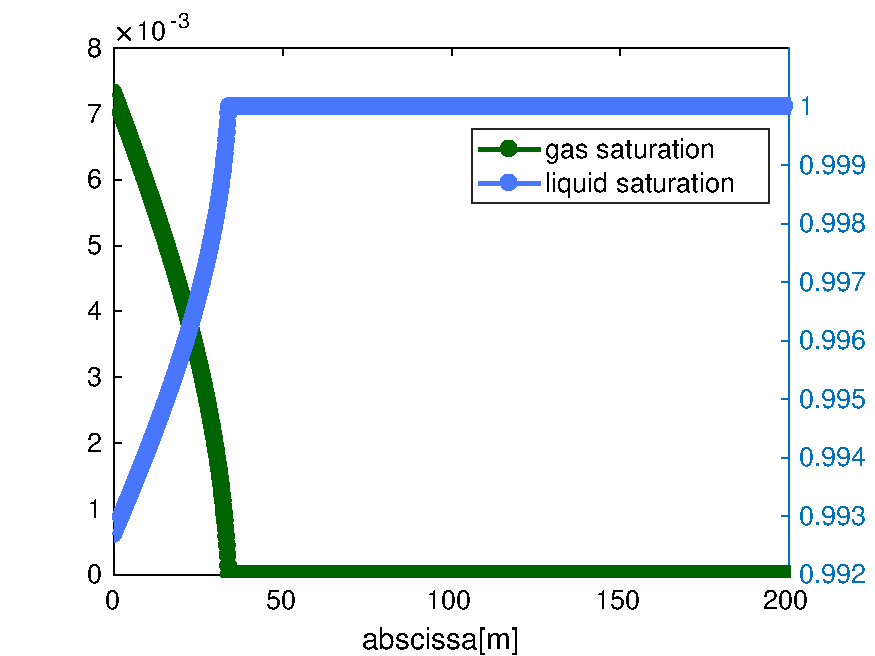
\includegraphics[width=\textwidth]{image/image_Jad/modif_saturations_cv_solver_1000_cells-eps-converted-to}    
\end{minipage}\hfill
\begin{minipage}[c]{.32\linewidth}
   \centering
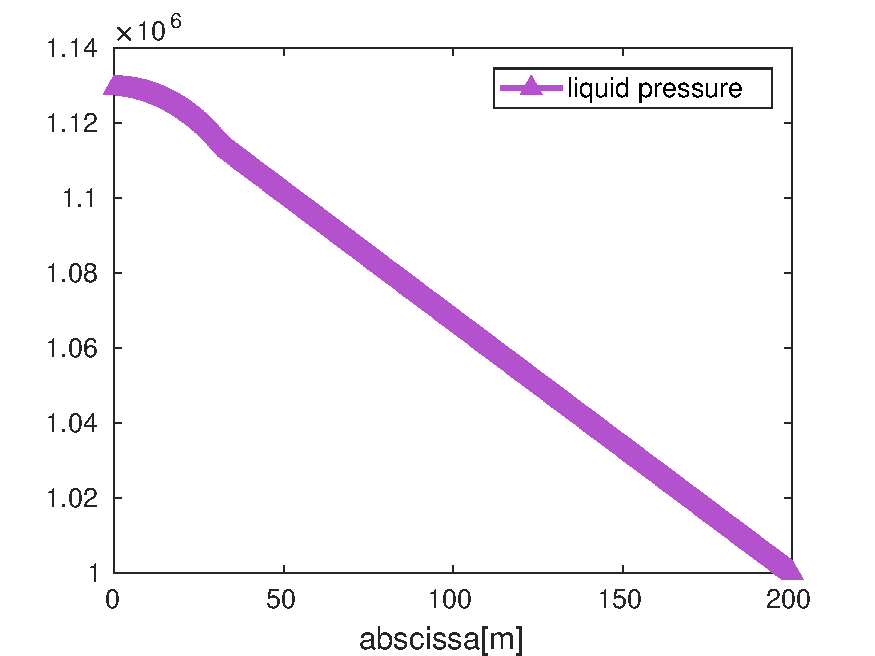
\includegraphics[width=\textwidth]{image/image_Jad/modif_liquid_pressure_cv_solver_1000_cells-eps-converted-to}    
\end{minipage}\hfill
\begin{minipage}[c]{.33\linewidth}
   \centering
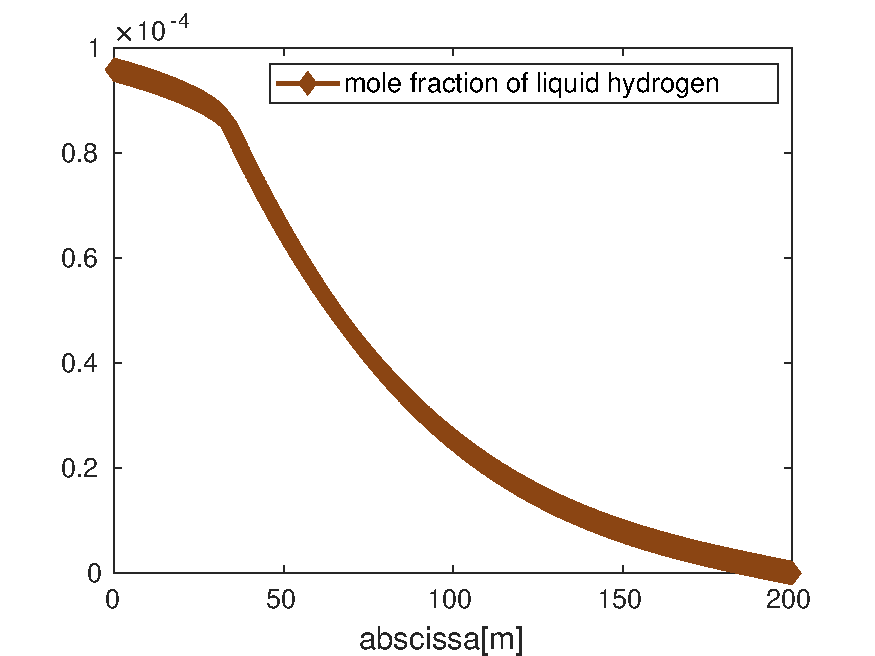
\includegraphics[width=\textwidth]{image/image_Jad/modif_mole_frac_cv_solver_1000_cells-eps-converted-to}     
\end{minipage}

\end{tcolorbox}
\begin{tcolorbox}
[enhanced, breakable,colback=white,frame style={left color=white!25!black,
right color=blue!75!black},
width=\dimexpr0.45\textwidth+18mm\relax,enlarge left by=0mm, title = \huge Bibliography, 
bottomrule=3mm, leftrule=1mm, toptitle = 3mm, bottomtitle = 3mm, center title]

{
\bibitem{Dabaghi:2017}
{\sc J.~Dabaghi, V.~Martin, and M.~Vohral{\'{\i}}k}, {\em Adaptive inexact
  semismooth Newton methods for the contact problem between two membranes}.
\textcolor{black}{submitted for publication, 2017.}
}

{
\bibitem{Dabaghi:2018}
{\sc I. Ben Gharbia, J.~Dabaghi, V.~Martin, and M.~Vohral{\'{\i}}k}, {\em A posteriori error estimates and stopping criteria for a two-phase flow with nonlinear complementarity constraints}.
\textcolor{black}{In preparation, 2018.}
}
\end{tcolorbox}


\begin{tcolorbox}
[enhanced, breakable,colback=white,frame style={left color=white!25!black,
right color=blue!75!black},
width=\dimexpr0.45\textwidth+18mm\relax,enlarge left by=0mm, title = \huge Weak solution, 
bottomrule=3mm, leftrule=1mm, toptitle = 3mm, bottomtitle = 3mm, center title]
%\textcolor{red}{\textbf{Function spaces}}
\begin{equation*}
X = L^2((0,\tF);H^1(\Omega)), \quad Y = H^1((0,\tF);L^2(\Omega)), \quad  Z = \left\{v \in L^2((0,\tF);L^2(\Omega)), \: v \geq 0  \right\}
\end{equation*}
\begin{assumption}[Weak formulation]
\begin{align*}
& \Pl, \Pg, \chihl \in X, \quad \Sl, \Sg, \lw, \lh,  \in Y \quad \left(\Phiw=\rhowl \darcyliq-\Jwl,  \Phih=\rhohl \darcyliq  + \rhohg \darcygas-\Jhl\right) \in [L^2((0,\tF); \HdivOmeg]^d,\\
%\label{eq:weak:formulation:1}
&\dps \int_{0}^{\tF} \left(\partial_t \lc, \varphi \right)_{\Omega}(t)\,\mathrm{dt}-\left(\Phic, \nab \varphi \right)_{\Omega}(t)\,\mathrm{dt}-\left(\Qc, \varphi \right)_{\Omega}(t)\,\mathrm{dt} = 0 \quad \forall \varphi \in X, \; \componentc=\componentw,\componenth,\\
%\label{eq:weak:formulation:2}
&\dps \int_{0}^{\tF} \left(\lambda-(\textcolor{electricpurple}{1 - \Sl}), \textcolor{carmine}{H \Pg-\betaliq \chihl}  \right)_{\Omega}(t)\,\mathrm{dt} \geq 0 \quad \forall \lambda \in Z, \quad \textcolor{electricpurple}{1 - \Sl} \in Z, \; \componentc=\componentw,\componenth ,\\
&\mbox{The initial condition, the algebraic closure relation, and Darcy's law hold}.
\end{align*}
\textcolor{black}{$\left\| \varphi \right\|_X = \left\{\sum_{n = 1}^{N_t} \int_{\In} \sum_{K \in \Th} \left(\varepsilon h_K^{-2} \left\|\varphi \right\|_K^2 +  \left\|\nab \varphi\right\|_{K}^2 \right) \, \mathrm{dt}  \right\}^\frac{1}{2}. \vspace{0.1 cm}$
}
\textcolor{black}{Define $\mathcal{C}^0$ and piecewise $\mathbb{P}_1$ in time and discontinous in space functions:} $\underbrace{\lchtaunki(\cdot,t^n)=\lchnki}_{\textcolor{cadmiumgreen}{\in \mathbb{P}_0(\Th)}}, \quad \underbrace{\Shtaunki(\cdot,t^n)=\Shnki}_{\textcolor{cadmiumgreen}{\in \mathbb{P}_0(\Th)}} \quad \underbrace{\Phtaunki(\cdot,t^n)=\Phnki}_{\textcolor{cadmiumgreen}{\in \mathbb{P}_2(\Th)}}, \quad \underbrace{\chihtaunki(\cdot,t^n)=\chihnki}_{\textcolor{cadmiumgreen}{\in \mathbb{P}_2(\Th)}}$
\end{assumption}
\end{tcolorbox}
%We equip the space $X$ with the norm 

\begin{tcolorbox}
[enhanced, breakable,colback=white,frame style={left color=white!25!black,
right color=blue!75!black},
width=\dimexpr0.45\textwidth+18mm\relax,enlarge left by=0mm, title = \huge Error measure, 
bottomrule=3mm, leftrule=1mm, toptitle = 3mm, bottomtitle = 3mm, center title]
\vspace{-0.2  cm}
\textcolor{cadmiumgreen}{\textbf{Dual norm of the residual for the components}}
\begin{equation*}
\hspace{-0.2 cm}\left\|\mathcal{R}_{\componentc}(\Shtaunki,\Phtaunki,\chihtaunki) \right\|_{X'} = \sup_{\varphi \in X, \left\|\varphi\right\|_X = 1} |\ \int_{0}^{\tF} 
\left(\Qc - \partial_t \lchtaunki , \varphi\right)_{\Omega}(t) + \left(\Phichtaunki,\nab \varphi \right)_{\Omega}(t)\,\mathrm{dt}|\ .
%\label{eq:dual:norm:residual}
\vspace{-0.25 cm}
\end{equation*}
\textcolor{cadmiumgreen}{\textbf{Residual for the constraints}}
\begin{equation*}
  \mathcal{R}_{\mathrm{e}}(\Shtaunki,\Phtaunki,\chihtaunki) = \int_{0}^{\tF}\left(\textcolor{electricpurple}{1 - \Shtaunki}, \textcolor{carmine}{H \left[\Phtaunki + \capillarypressure(\Shtaunki)\right] - \betaliq \chihtaunki} \right)_{\Omega}(t)\,\mathrm{dt}.
\end{equation*}
\vspace{-0.3 cm} 
\textcolor{cadmiumgreen}{\textbf{Distance of the pressure $\Phtaunki$ to the space $X$ (nonconformity of the pressure)}}
\begin{equation*}
\mathcal{N}_{\phasep}^{n,\textcolor{royalblue}{k},\textcolor{burntorange}{i}} = \inf_{\delta_{\phasep}^{n,\textcolor{royalblue}{k},\textcolor{burntorange}{i}} \in X} 
\left\{
\sum_{\componentc \in \mathcal{C}_{\phasep}}
 \int_{0}^{\tF} \left\|\mu_{\phasep}^{-1}k_{r \phasep}(\Sp) \rho_{\componentc}^{\phasep} \tensor \nab \left(\Phtaunki-\delta_{\phasep}^{n,\textcolor{royalblue}{k},\textcolor{burntorange}{i}}\right)(t) \right\|^2 \,\mathrm{dt} 
\right\}^{\frac{1}{2}}, 
\vspace{-0.15 cm}
\end{equation*}
\vspace{-0.15 cm}
\textcolor{cadmiumgreen}{\textbf{Distance of the mole fraction $\chihtaunki$ to the space $X$ (nonconformity of the mole fraction)}}
\vspace{-0.2 cm}
\begin{equation*}
\mathcal{N}_{\chi}^{n,\textcolor{royalblue}{k},\textcolor{burntorange}{i}}:=\inf_{\theta^{n,\textcolor{royalblue}{k},\textcolor{burntorange}{i}} \in X} \left\{\int_{0}^{\tF} \left\|- M^{\componenth} \Shtaunki \left(\rhowl/M^{\componentw} + \betaliq /M^{\componenth} \chihnki \right) D_{\componenth}^{\phasel} {\bm \nabla}(\chihtaunki - \theta^{n,\textcolor{royalblue}{k},\textcolor{burntorange}{i}})(t)\right\|^2\,\mathrm{dt} \right\}^\frac{1}{2},
\end{equation*}
\vspace{-0.5 cm}
\textcolor{cadmiumgreen}{\textbf{Error measure}}
$ \dps \mathcal{N}^{n,\textcolor{royalblue}{k},\textcolor{burntorange}{i}} := \left\{\sum_{\componentc \in\mathcal{C}} \left\|\mathcal{R}_{\componentc}(\Shtaunki,\Phtaunki,\chihtaunki) \right\|_{X'}^2 \right\}^{\frac{1}{2}} + \left\{\sum_{\phasep \in \mathcal{P}} \left(\Npnki\right)^2 + \left(\Nchinki\right)^2\right\}^{\frac{1}{2}} + \mathcal{R}_{\mathrm{e}}(\Shtaunki,\Phtaunki,\chihtaunki).
$ 
% \begin{definition}[Error measure]
% \vspace{-0.5 cm}
% \begin{equation*}
%   \mathcal{N}^{n,\textcolor{royalblue}{k},\textcolor{burntorange}{i}} = \left\{\sum_{\componentc \in\mathcal{C}} \left\|\mathcal{R}_{\componentc}(\Shtaunki,\Phtaunki,\chihtaunki) \right\|_{X'}^2 \right\}^{\frac{1}{2}} + \left\{\sum_{\phasep \in \mathcal{P}} \left(\Npnki\right)^2 + \left(\Nchinki\right)^2\right\}^{\frac{1}{2}} + \mathcal{R}_{\mathrm{e}}(\Shtaunki,\Phtaunki,\chihtaunki)
% \label{eq:norm:aposteriori}
% \end{equation*}
% \end{definition}
\end{tcolorbox}
\begin{tcolorbox}
[enhanced, breakable,colback=white,frame style={left color=white!25!black,
right color=blue!75!black},
width=\dimexpr0.45\textwidth+18mm\relax,enlarge left by=0mm, title = \huge Reconstruction, 
bottomrule=3mm, leftrule=1mm, toptitle = 3mm, bottomtitle = 3mm, center title]
\begin{minipage}{0.4 \linewidth}
 % \hspace{4 cm}\textcolor{blue}{\textbf{$ \bm H^1$ pressure reconstruction}}
  $\Nsp=3$
  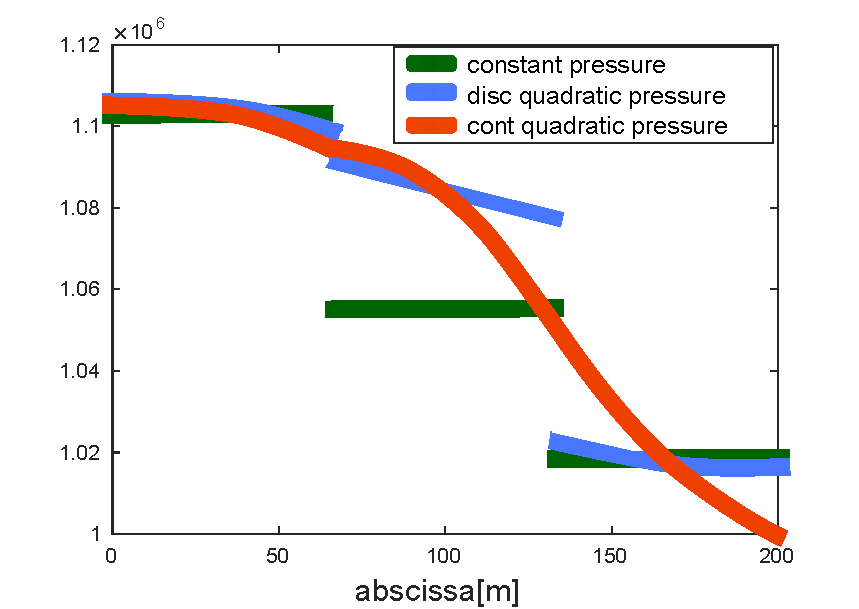
\includegraphics[width=0.8\textwidth]{image/image_Jad/modif_image_post_process_cont}  
\end{minipage}
\hfill
\begin{minipage}{0.6\linewidth}
  \hspace*{2.5 cm}\textcolor{red}{\textbf{\large{Component flux reconstruction}}}\\
\textcolor{cadmiumgreen}{\textbf{Discretization flux:}}
$\left(\Thetachdiscnki \cdot \bn_K,1 \right)_{\sigma} = F_{\componentc,K,\sigma}\left(\bU^{n,\textcolor{royalblue}{k}, \textcolor{burntorange}{i}}\right)$,\\
\textcolor{cadmiumgreen}{\textbf{Linearization flux:}}
$\left(\Thetachlinnki \cdot \bn_K,1 \right)_{\sigma} = \FcKsigmanki -  F_{\componentc,K,\sigma}\left(\bU^{n,\textcolor{royalblue}{k}, \textcolor{burntorange}{i}}\right),$\\
\textcolor{cadmiumgreen}{\textbf{Algebraic flux:}}$
\left(\Thetachalgnki \cdot \bn_K,1 \right)_{\partial K} = - {\bR}_{\componentc,K}^{n,\textcolor{royalblue}{k}, \textcolor{burntorange}{i}}$,\\
\textcolor{cadmiumgreen}{\textbf{Total flux:}} 
$\Thetachnki = \Thetachdiscnki+\Thetachlinnki+\Thetachalgnki
$.
\end{minipage}

\end{tcolorbox}
\begin{tcolorbox}
[enhanced, breakable,colback=white,frame style={left color=white!25!black,
right color=blue!75!black},
width=\dimexpr0.45\textwidth+18mm\relax,enlarge left by=0mm, title = \huge Error estimators, 
bottomrule=3mm, leftrule=1mm, toptitle = 3mm, bottomtitle = 3mm, center title]
\textcolor{cadmiumgreen}{Discretization estimators}
$$
 \left.
    \begin{array}{ll}
   \etaFKcnki(t) = \left\|\Thetachnki - \Phichtaunki(t) \right\|_K, \quad \etaPKposnki(t)=\left(\left\{1-\Shtaunki\right\}^{+}(t),\left\{H\left[\Phtaunki \hspace{-0.1 cm}+\hspace{-0.1 cm} \capillarypressure\left(\Shtaunki\right)\right]\hspace{-0.1 cm}-\betaliq \chihtaunki\right\}^{+}(t)\right)_K,\\
\etaRKcnki = \min\left\{\CPW,\varepsilon^{-\frac{1}{2}}\right\} h_K \left\|\Qchn - \frac{\lcK(\bU^{n,\textcolor{royalblue}{k}-1}) - \lcK^{n-1} + \LcKnki}{\Tn} - \nab \cdot \Thetachnki \right\|_K \vspace{0.2 cm},\\

      \etaNCKpcnki(t) = \left\|\frac{k_{r \phasel}(\Sl)}{\mu_{\phasel}} \rho_{\componentc}^{\phasep} \tensor \nab(\Phtaupnki-I_{\mathrm{os}}(\Phpnki))(t)\right\|_K,    
\end{array} 
\right.
$$
%
\begin{minipage}{0.9 \linewidth}
\textcolor{cadmiumgreen}{Linearization estimators}
$$
 \left.
    \begin{array}{ll}
\etaNAKcnki  = \varepsilon^{-\frac{1}{2}} h_K \left(\Tn\right)^{-1} \left\|\lcK(\bU^{n,\textcolor{royalblue}{k},\textcolor{burntorange}{i}}) - \lcK(\bU^{n,\textcolor{royalblue}{k}-1}) - \LcKnki \right\|_K,\\
\etaPKnegnki(t)  = \left(\left\{1 - \Shtaunki\right\}^{-}\hspace{-0.2 cm}(t),\left\{H\left[\Phtaunki + \capillarypressure\left(\Shtaunki\right)\right]-\betaliq \chihtaunki\right\}^{-}(t)\right)_K,
 \end{array}
$$
\end{minipage}
\hfill
\begin{minipage}{0.3 \linewidth}
\textcolor{cadmiumgreen}{Algebraic estimator}
\begin{equation*}
\etaalgKcnki=\left\|\Thetachalgnki\right\|_K,  \hspace{7 cm} \boxed{\mathcal{N}^{n,\textcolor{royalblue}{k},\textcolor{burntorange}{i}}\leq \etadiscnki + \etalinnki + \etaalgnki}
\end{equation*}
\end{minipage}
% \begin{theorem}
% \begin{equation*}
% %\label{eq:corrolary:component:error}
% \mathcal{N}^n \leq \etadiscnki + \etalinnki + \etaalgnki
% \end{equation*}  
%\end{theorem}
\end{tcolorbox}
\begin{tcolorbox}
[enhanced, breakable,colback=white,frame style={left color=white!25!black,
right color=blue!75!black},
width=\dimexpr0.45\textwidth+18mm\relax,enlarge left by=0mm, title = \huge Adaptivity, 
bottomrule=3mm, leftrule=1mm, toptitle = 3mm, bottomtitle = 3mm, center title]
\textcolor{cadmiumgreen}{\textbf{Stopping criterion algebraic solver:}}  \hspace{-0.3 cm}\fcolorbox{violet}{white}{$\eta_{\mathrm{alg}}^{n,\textcolor{royalblue}{k},\textcolor{burntorange}{i}} \leq \gamma_{\mathrm{alg}} \max  \left\{{\eta_{\mathrm{disc}}^{n,\textcolor{royalblue}{k},\textcolor{burntorange}{i}}, \eta_{\mathrm{lin}}^{n,\textcolor{royalblue}{k},\textcolor{burntorange}{i}}}\right\}$}\\
\textcolor{cadmiumgreen}{\textbf{Stopping criterion linear solver:}} \fcolorbox{violet}{white}{ $\eta_{\mathrm{lin}}^{n,\textcolor{royalblue}{k},\textcolor{burntorange}{i}} \leq \gamma_{\mathrm{lin}} \eta_{\mathrm{disc}}^{n,\textcolor{royalblue}{k},\textcolor{burntorange}{i}}$}\\
\begin{minipage}{0.5 \linewidth}
  \centering
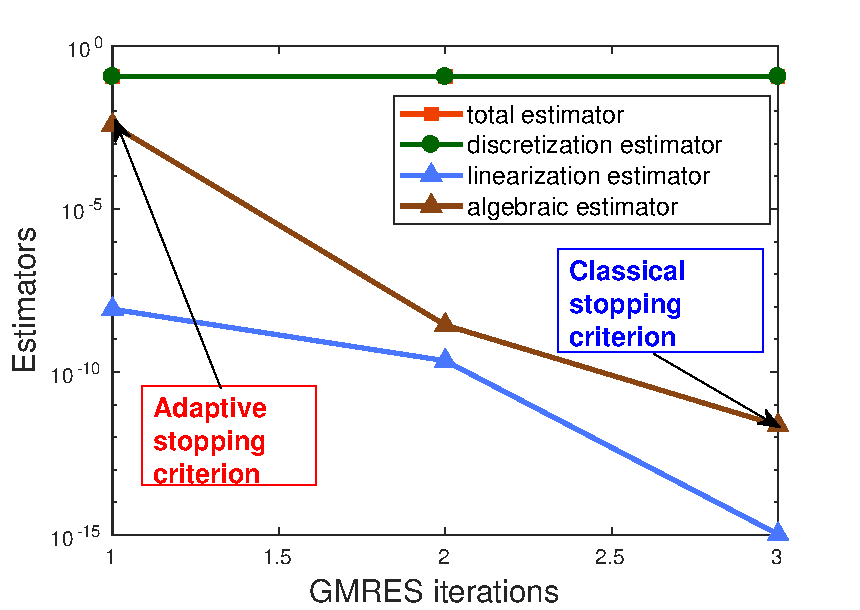
\includegraphics[width=0.65\textwidth]{image/image_Jad/modif_picture_estimators_two_phase_gmres}
\end{minipage}
\hfill
\begin{minipage}{0.5 \linewidth}
\centering
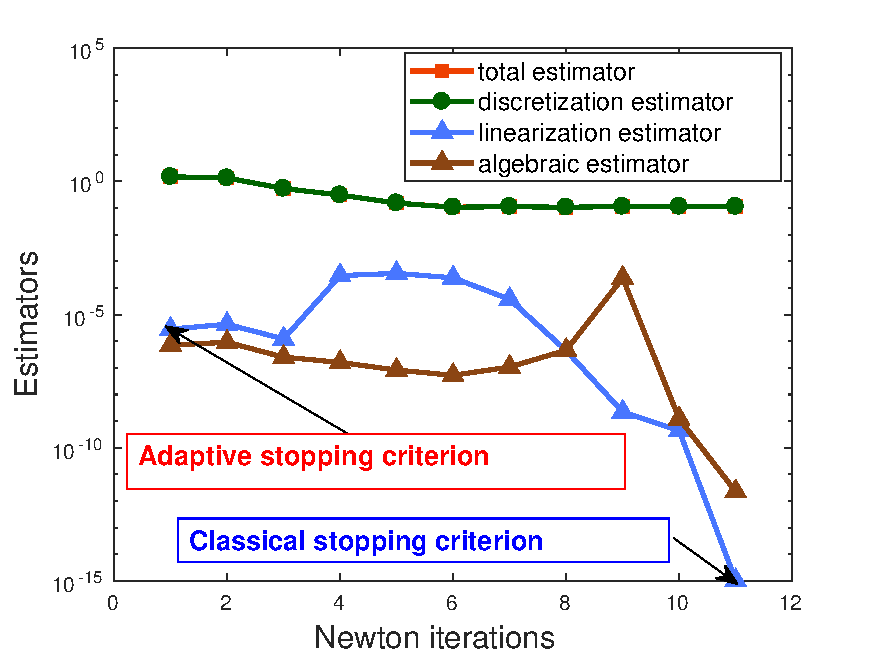
\includegraphics[width=0.65\textwidth]{image/image_Jad/modif_picture_estimators_two_phase}
\end{minipage}    
\end{tcolorbox}


\end{multicols}
\end{document}
